\let\negmedspace\undefined
\let\negthickspace\undefined
\documentclass[journal]{IEEEtran}
\usepackage[a5paper, margin=10mm, onecolumn]{geometry}
%\usepackage{lmodern} % Ensure lmodern is loaded for pdflatex
\usepackage{tfrupee} % Include tfrupee package

\setlength{\headheight}{1cm} % Set the height of the header box
\setlength{\headsep}{0mm}     % Set the distance between the header box and the top of the text
\usepackage{multicol}
\usepackage{gvv-book}
\usepackage{gvv}
\usepackage{cite}
\usepackage{amsmath,amssymb,amsfonts,amsthm}
\usepackage{algorithmic}
\usepackage{graphicx}
\usepackage{textcomp}
\usepackage{xcolor}
\usepackage{txfonts}
\usepackage{listings}
\usepackage{enumitem}
\usepackage{mathtools}
\usepackage{gensymb}
\usepackage{comment}
\usepackage[breaklinks=true]{hyperref}
\usepackage{tkz-euclide} 
\usepackage{listings}
% \usepackage{gvv}                                        
\def\inputGnumericTable{}                                 
\usepackage[latin1]{inputenc}                                
\usepackage{color}                                            
\usepackage{array}                                            
\usepackage{longtable}                                       
\usepackage{calc}                                             
\usepackage{multirow}                                         
\usepackage{hhline}                                           
\usepackage{ifthen}                                           
\usepackage{lscape}
\usepackage{tikz}
\usepackage{tikz-3dplot}
\begin{document}

\bibliographystyle{IEEEtran}
\vspace{3cm}

\title{2011-PH}
\author{EE24BTECH11027 - satwikagv}
% \maketitle
% \newpage
% \bigskip
{\let\newpage\relax\maketitle}

\renewcommand{\thefigure}{\theenumi}
\renewcommand{\thetable}{\theenumi}
\setlength{\intextsep}{10pt} % Space between text and floats


\numberwithin{equation}{enumi}
\numberwithin{figure}{enumi}
\renewcommand{\thetable}{\theenumi}
\begin{enumerate}
	\item Consider a cylinder of height $h$ and radius $a$, closed at both ends, centered at the origin. Let $\vec{r}=\hat{i}x+\hat{j}y+\hat{k}z$ be the position vector and $\hat{n}$ a vector normal to the surface. The surface integral $\displaystyle \int\limits_{S} \vec{r}\cdot \hat{n}$ ds
over the closed surface of the cylinder is
\begin{tikzpicture}
\draw[thick] (0,0) ellipse (1 and 0.5);
\draw[thick] (0,-2) ellipse (1 and 0.5);
\draw[thick] (1,0) -- (1,-2);
\draw[thick] (-1,0) -- (-1,-2);
\filldraw[black] (0,-1) circle (1pt) node[anchor=north east] {$O$};
\draw[->, thick] (0,-1) -- (3,-1) node[anchor=west] {$y$};
\draw[->, thick] (0,-1) -- (0,1) node[anchor=north] {$z$};
\draw[->, thick] (0,-1) -- (-2.5,-2) node[anchor=north east] {$x$};
\end{tikzpicture}
\begin{multicols}{2}
\begin{enumerate}
    \item $2\pi a^2\brak{a+h}$
    \item $3\pi a^2h$
    \item $2\pi a^2h$
    \item zero
\end{enumerate}
\end{multicols}
\item The solutions to the differential equation 
\begin{align*}
\frac{dy}{dx}=-\frac{x}{y+1}
\end{align*}
 are a family of
\begin{enumerate}
    \item circles with different radii
    \item circles with different centres
    \item straight lines with different slopes
    \item straight lines with different intercepts on the $y$-axis
\end{enumerate}
\item A particle is moving under the action of a generalized potential
\begin{align*}
    V\brak{q,\dot{q}}=\frac{1+\dot{q}}{q^2}
\end{align*}
The magnitude of the generalized force is
\begin{multicols}{4}
    \begin{enumerate}
        \item $\frac{2\brak{1+\dot{q}}}{q^3}$
        \item $\frac{2\brak{1-\dot{q}}}{q^3}$
        \item $\frac{2}{q^3}$
        \item $\frac{\dot{q}}{q^3}$
    \end{enumerate}
\end{multicols}
\item Two bodies mass $m$ and $2m$ are connected by a spring of spring constant $k$. The frequency of the normal mode is
\begin{multicols}{4}
    \begin{enumerate}
        \item $\sqrt{\frac{3k}{2m}}$
        \item $\sqrt{\frac{k}{m}}$
        \item $\sqrt{\frac{2k}{3m}}$
        \item $\sqrt{\frac{k}{2m}}$
    \end{enumerate}
\end{multicols}
\item Let \brak{p,q} and \brak{P,Q} be two pairs of canonical variables. The transformation
\begin{align*}
    Q=q^{\alpha}\cos{\beta p}\\
    P=q^{\alpha}\sin{\beta p} 
\end{align*}
is canonical for
\begin{multicols}{4}
    \begin{enumerate}
        \item $\alpha =2, \beta =\frac{1}{2}$
        \item $\alpha =2, \beta =2$
        \item $\alpha =1, \beta =1$
        \item $\alpha =\frac{1}{2}, \beta =2$
    \end{enumerate}
\end{multicols}
\item Two particles, each of rest mass $m$ collide head-on and stick together. Before collision, the speed of each, mass was 0.6 times the speed of light in free space. The mass of the final entity is
\begin{multicols}{4}
    \begin{enumerate}
        \item $\frac{5m}{4}$
        \item $2m$
        \item $\frac{5m}{2}$
        \item $\frac{25m}{8}$
    \end{enumerate}
\end{multicols}
\item The normalized eigenstate of a particle in a one-dimensional potential well
\begin{align*}
    V\brak{x}=
    \begin{cases}
    0 & \text{ if } 0 \le x \le a \\ \infty & \text{otherwise}
    \end{cases}
\end{align*}
are given by
\begin{align*}
    \psi_n\brak{x}=\sqrt{\frac{2}{a}}\sin\brak{\frac{n\pi x}{a}} , \quad \text{ where } n=1,2,3\dots
\end{align*}
The particle is subjected to a perturbation
\begin{align*}
V^\prime \brak{x}=
    \begin{cases}
    V_0\cos{\frac{\pi x}{a}} & \text{  for }0 \le x \le \frac{a}{2}
    \\ 0 & \text{\space otherwise}
    \end{cases}
\end{align*}
The shift in the ground state energy due to the perturbation, in the first order perturbation theory, is
\begin{multicols}{4}
    \begin{enumerate}
        \item $\frac{2V_0}{3\pi}$
        \item $\frac{V_0}{3\pi}$
        \item $-\frac{V_0}{3\pi}$
        \item $-\frac{2V_0}{3\pi}$
    \end{enumerate}
\end{multicols}
\item If the isothermal compressibility of a solid is $K_T = 10^{-10} \brak{\text{Pa}}^{-1}$, the pressure required to increase its density by 1\% is approximately
\begin{multicols}{4}
    \begin{enumerate}
        \item $10^4$ Pa
        \item $10^6$ Pa
        \item $10^8$ Pa
        \item $10^{10}$ Pa
    \end{enumerate}
\end{multicols}
\item A system of $N$ non-interacting and distinguishable particles of spin 1 is in thermodynamic equilibrium. The entropy of the system is
\begin{multicols}{4}
    \begin{enumerate}
        \item $2k_B \ln N$
        \item $3k_B \ln N$
        \item $Nk_B \ln 2$
        \item $Nk_B \ln 3$
    \end{enumerate}
\end{multicols}
\item A system has two energy levels with energies $\epsilon$ and $2\epsilon$. The lower level is 4-fold-degenerate while the upper level is doubly degenerate. If there are $N$ non-interacting classical particles in the system, which is in thermodynamic equilibrium at a temperature $T$, the fraction of particles in the upper level is
\begin{multicols}{2}
    \begin{enumerate}
        \item $\frac{1}{1+e^{-\frac{\epsilon}{k_BT}}}$
        \item $\frac{1}{1+2e^{\frac{\epsilon}{k_BT}}}$
        \item $\frac{1}{2e^{\frac{\epsilon}{k_BT}}+e^{\frac{2\epsilon}{k_BT}}}$
        \item $\frac{1}{2e^{\frac{\epsilon}{k_BT}}-e^{\frac{2\epsilon}{k_BT}}}$
    \end{enumerate}
\end{multicols}
\item A spherical conductor of radius $a$ is placed in a uniform electric field $\vec{E}=E_0\hat{k}$. The potential at a point $\vec{P}\brak{r,\theta}$ for $ r>a $, is given by
\begin{align*}
    \pi \brak{r,\theta}=constant-E_0r\cos\theta +\frac{E_0a^3}{r^2}\cos\theta
\end{align*}
where $r$ is the distance of $\vec{P}$ from the centre $\vec{O}$ of the sphere and $\theta$ is the angle $OP$ with the $z$-axis.
\begin{tikzpicture}
     \draw[thick] (0,0) circle (1);
     \filldraw[black] (0,0) circle (1pt) node[anchor=north east] {$ O $};
     \coordinate (P) at (0.75, 1.5);
     \filldraw[black] (P) circle (1pt) node[anchor=south west] {$P$};
	\draw[thick, -] (0,0) -- (P) node[midway, anchor=east] {$r$};
     \draw[thick, -] (0,0) -- (P);
     \draw[thick, ->] (0,0) -- (2,0) node[anchor=west] {$\hat{k}$};
     \draw[thick] (0.5, 0) arc[start angle=0, end angle=63.4, radius=0.5];
     \node at (0.8, 0.3) {$\theta$};
\end{tikzpicture}
\\The charge density of the sphere at $\theta = 30\degree$ is
\begin{multicols}{4}
    \begin{enumerate}
        \item $\frac{3\sqrt{3}\epsilon_0E_0}{2}$
        \item $\frac{3\epsilon_0E_0}{2}$
        \item $\frac{\sqrt{3}\epsilon_0E_0}{2}$
        \item $\frac{\epsilon_0E_0}{2}$
    \end{enumerate}
\end{multicols}
\item According to the single particle nuclear shell model, the spin-parity of the ground state of $\prescript{17}{8}{O}$ is
\begin{multicols}{4}
    \begin{enumerate}
        \item $\frac{1}{2}^-$
        \item $\frac{3}{2}^-$
        \item $\frac{3}{2}^+$
        \item $\frac{5}{2}^+$
    \end{enumerate}
\end{multicols}
\item In the $\beta$-decay of neutron $n\rightarrow p+e^-+V_e$, the anti-neutrino $V_e$ escapes detection. Its existence is inferred from the measurement of
\begin{enumerate}
    \item energy distribution of electrons
    \item angular distribution of electrons
    \item helicity distribution of electrons 
    \item forward-backward asymmetry of electrons
\end{enumerate}
\end{enumerate}
\end{document}
